\section{Results}

\subsection{LASA Handwriting Dataset}
We used the LASA handwriting dataset which consists of a library of 2D handwriting motion trajectories~\cite{Khansari-Zadeh11tro}. There are 7 trajectories recorded for each handwriting motion. All the trajectories of a given hand motion start from different positions but end at the same position. Each trajectory consists of a set of states consisting of timestamp, $x$-position, $y$-position, $x$-velocity, $y$-velocity, $x$-acceleration, and $y$-acceleration. We are primarily interested in learning the position values for each timestamp along the trajectory because we can derive the velocity from the positions. Our framework was tested with the 'heee' handwriting motion.

\begin{figure*}[h!]
	\captionsetup{font=footnotesize}
	\centering

	\begin{subfigure}{0.45\textwidth}
		\label{fig:atlasrobot}
	    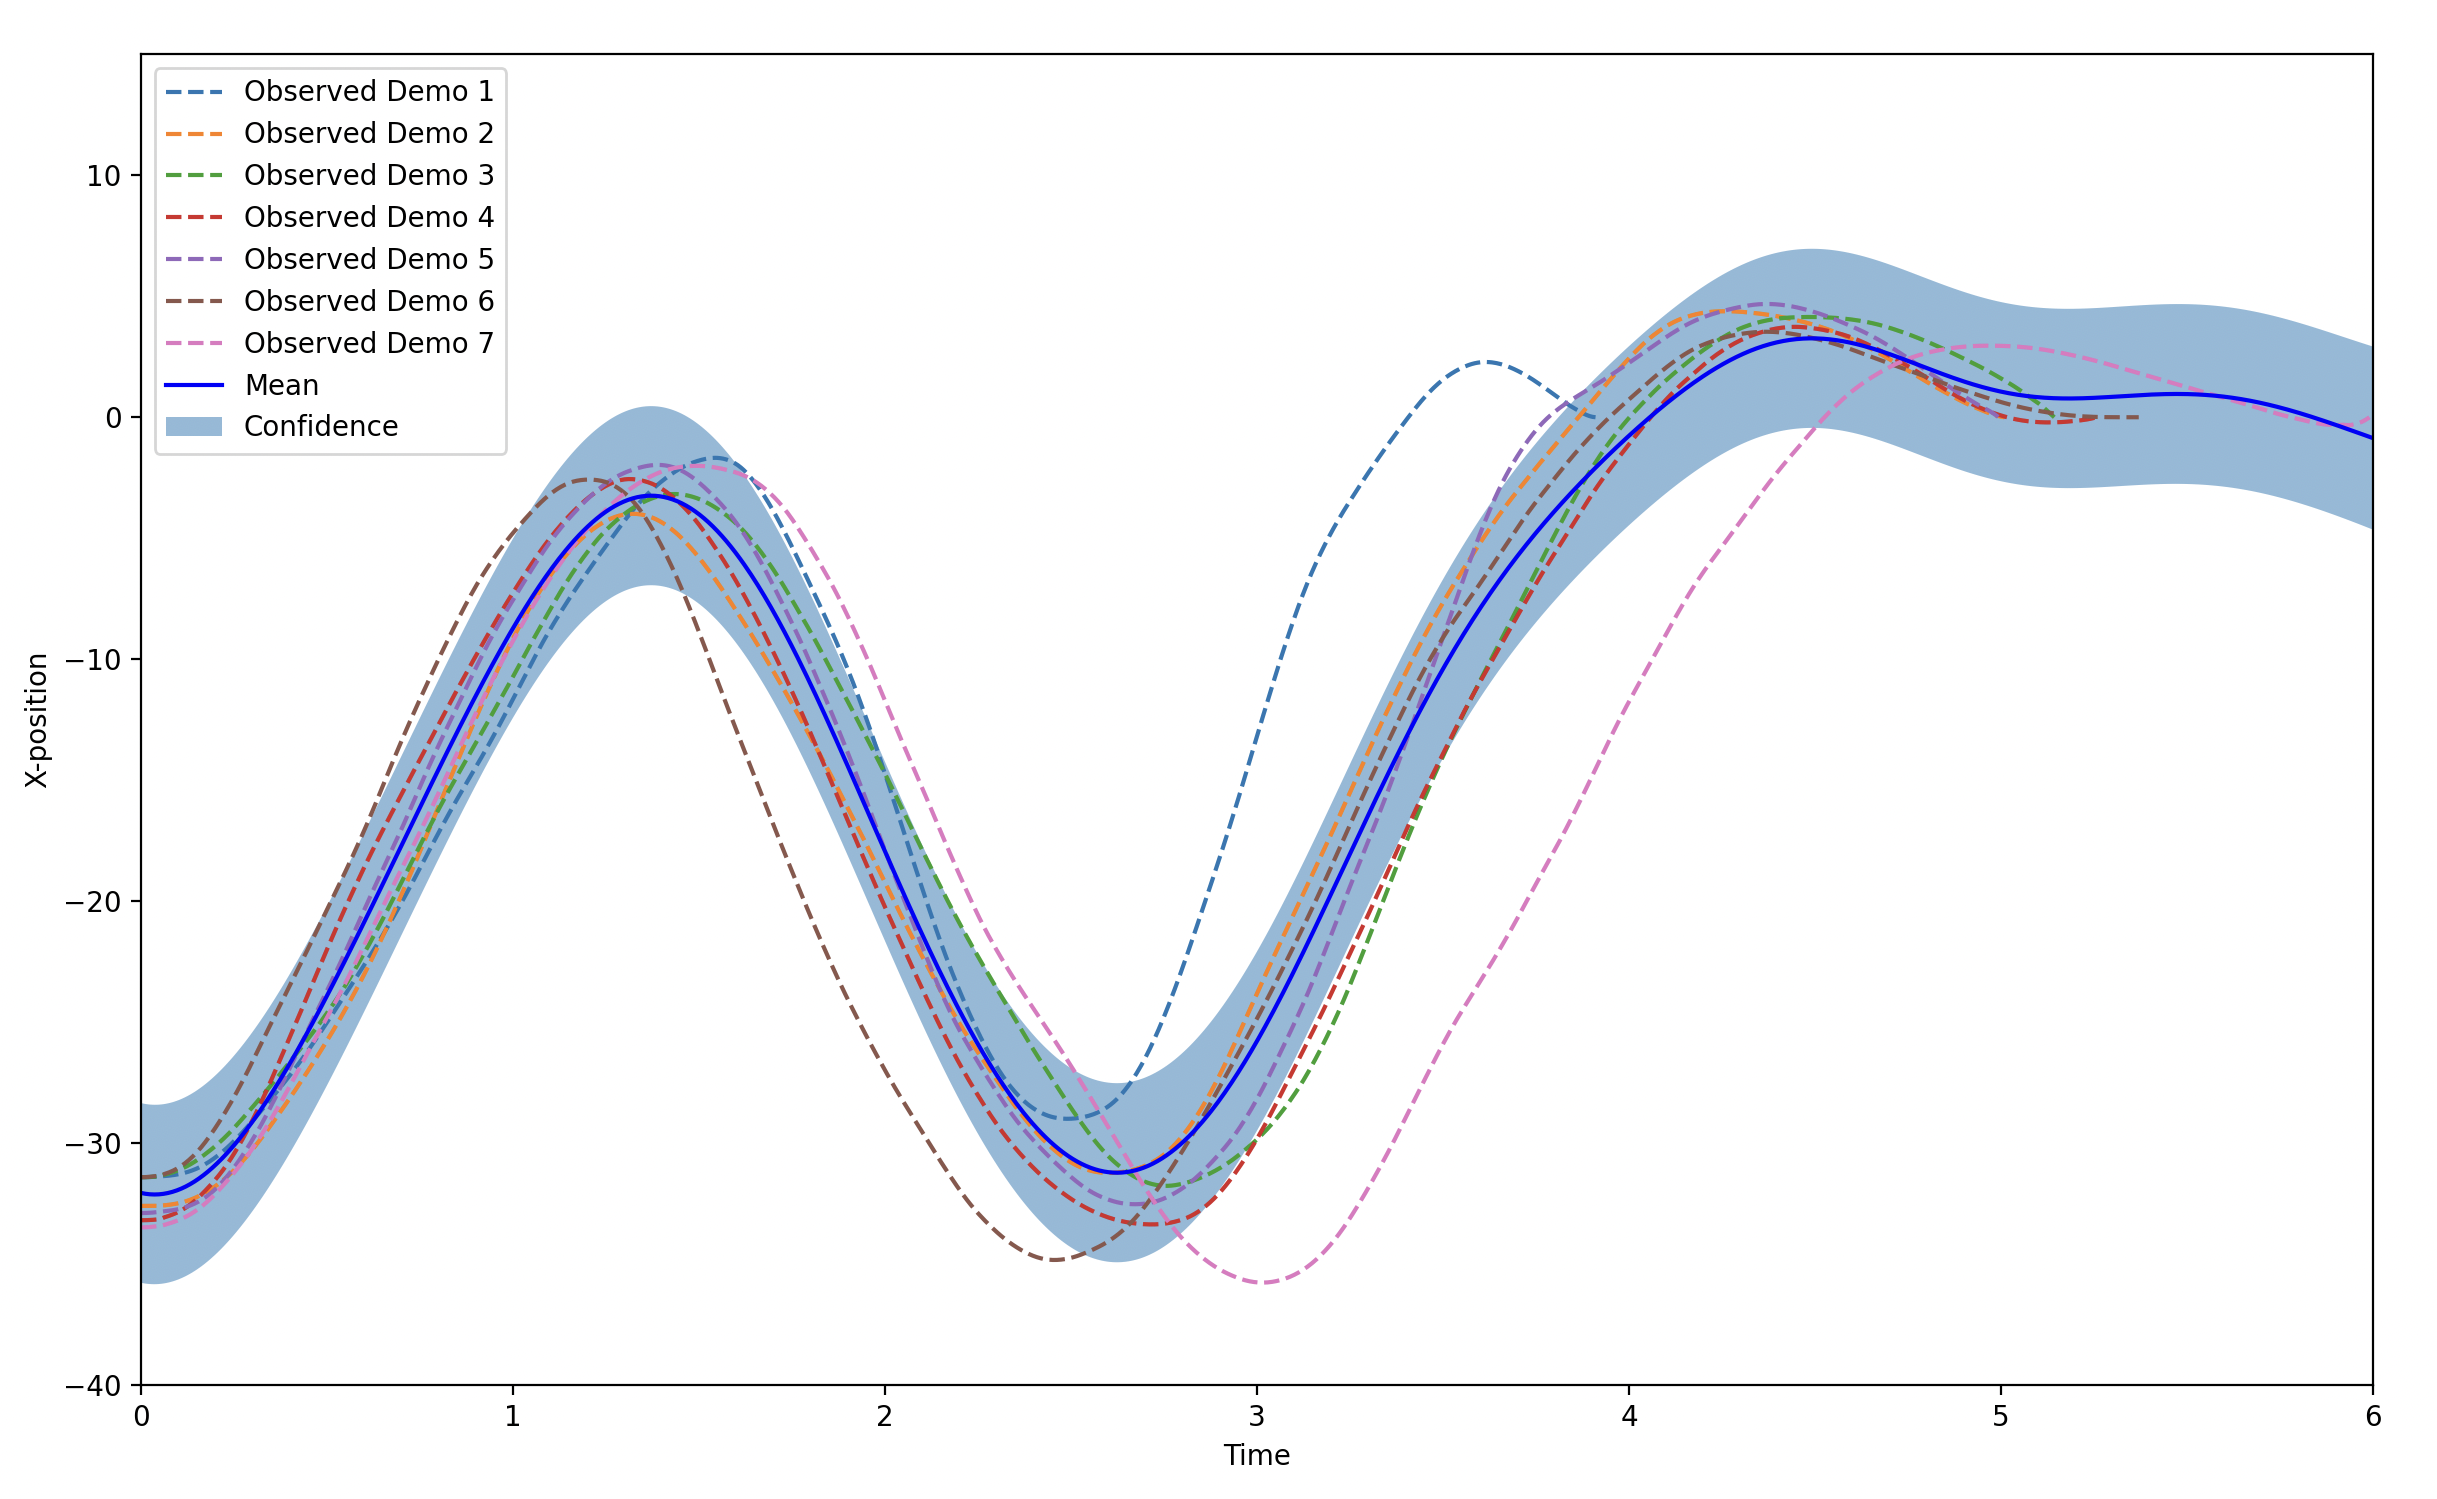
\includegraphics[width=\textwidth]{paper/images/X_time_Exact_GP_RBF.png}
		\caption{$x$ position as the task (output) and time $t$ as the input to the GP.}
	\end{subfigure}
	\begin{subfigure}{0.45\textwidth}
		\label{fig:atlas_traj_example}
		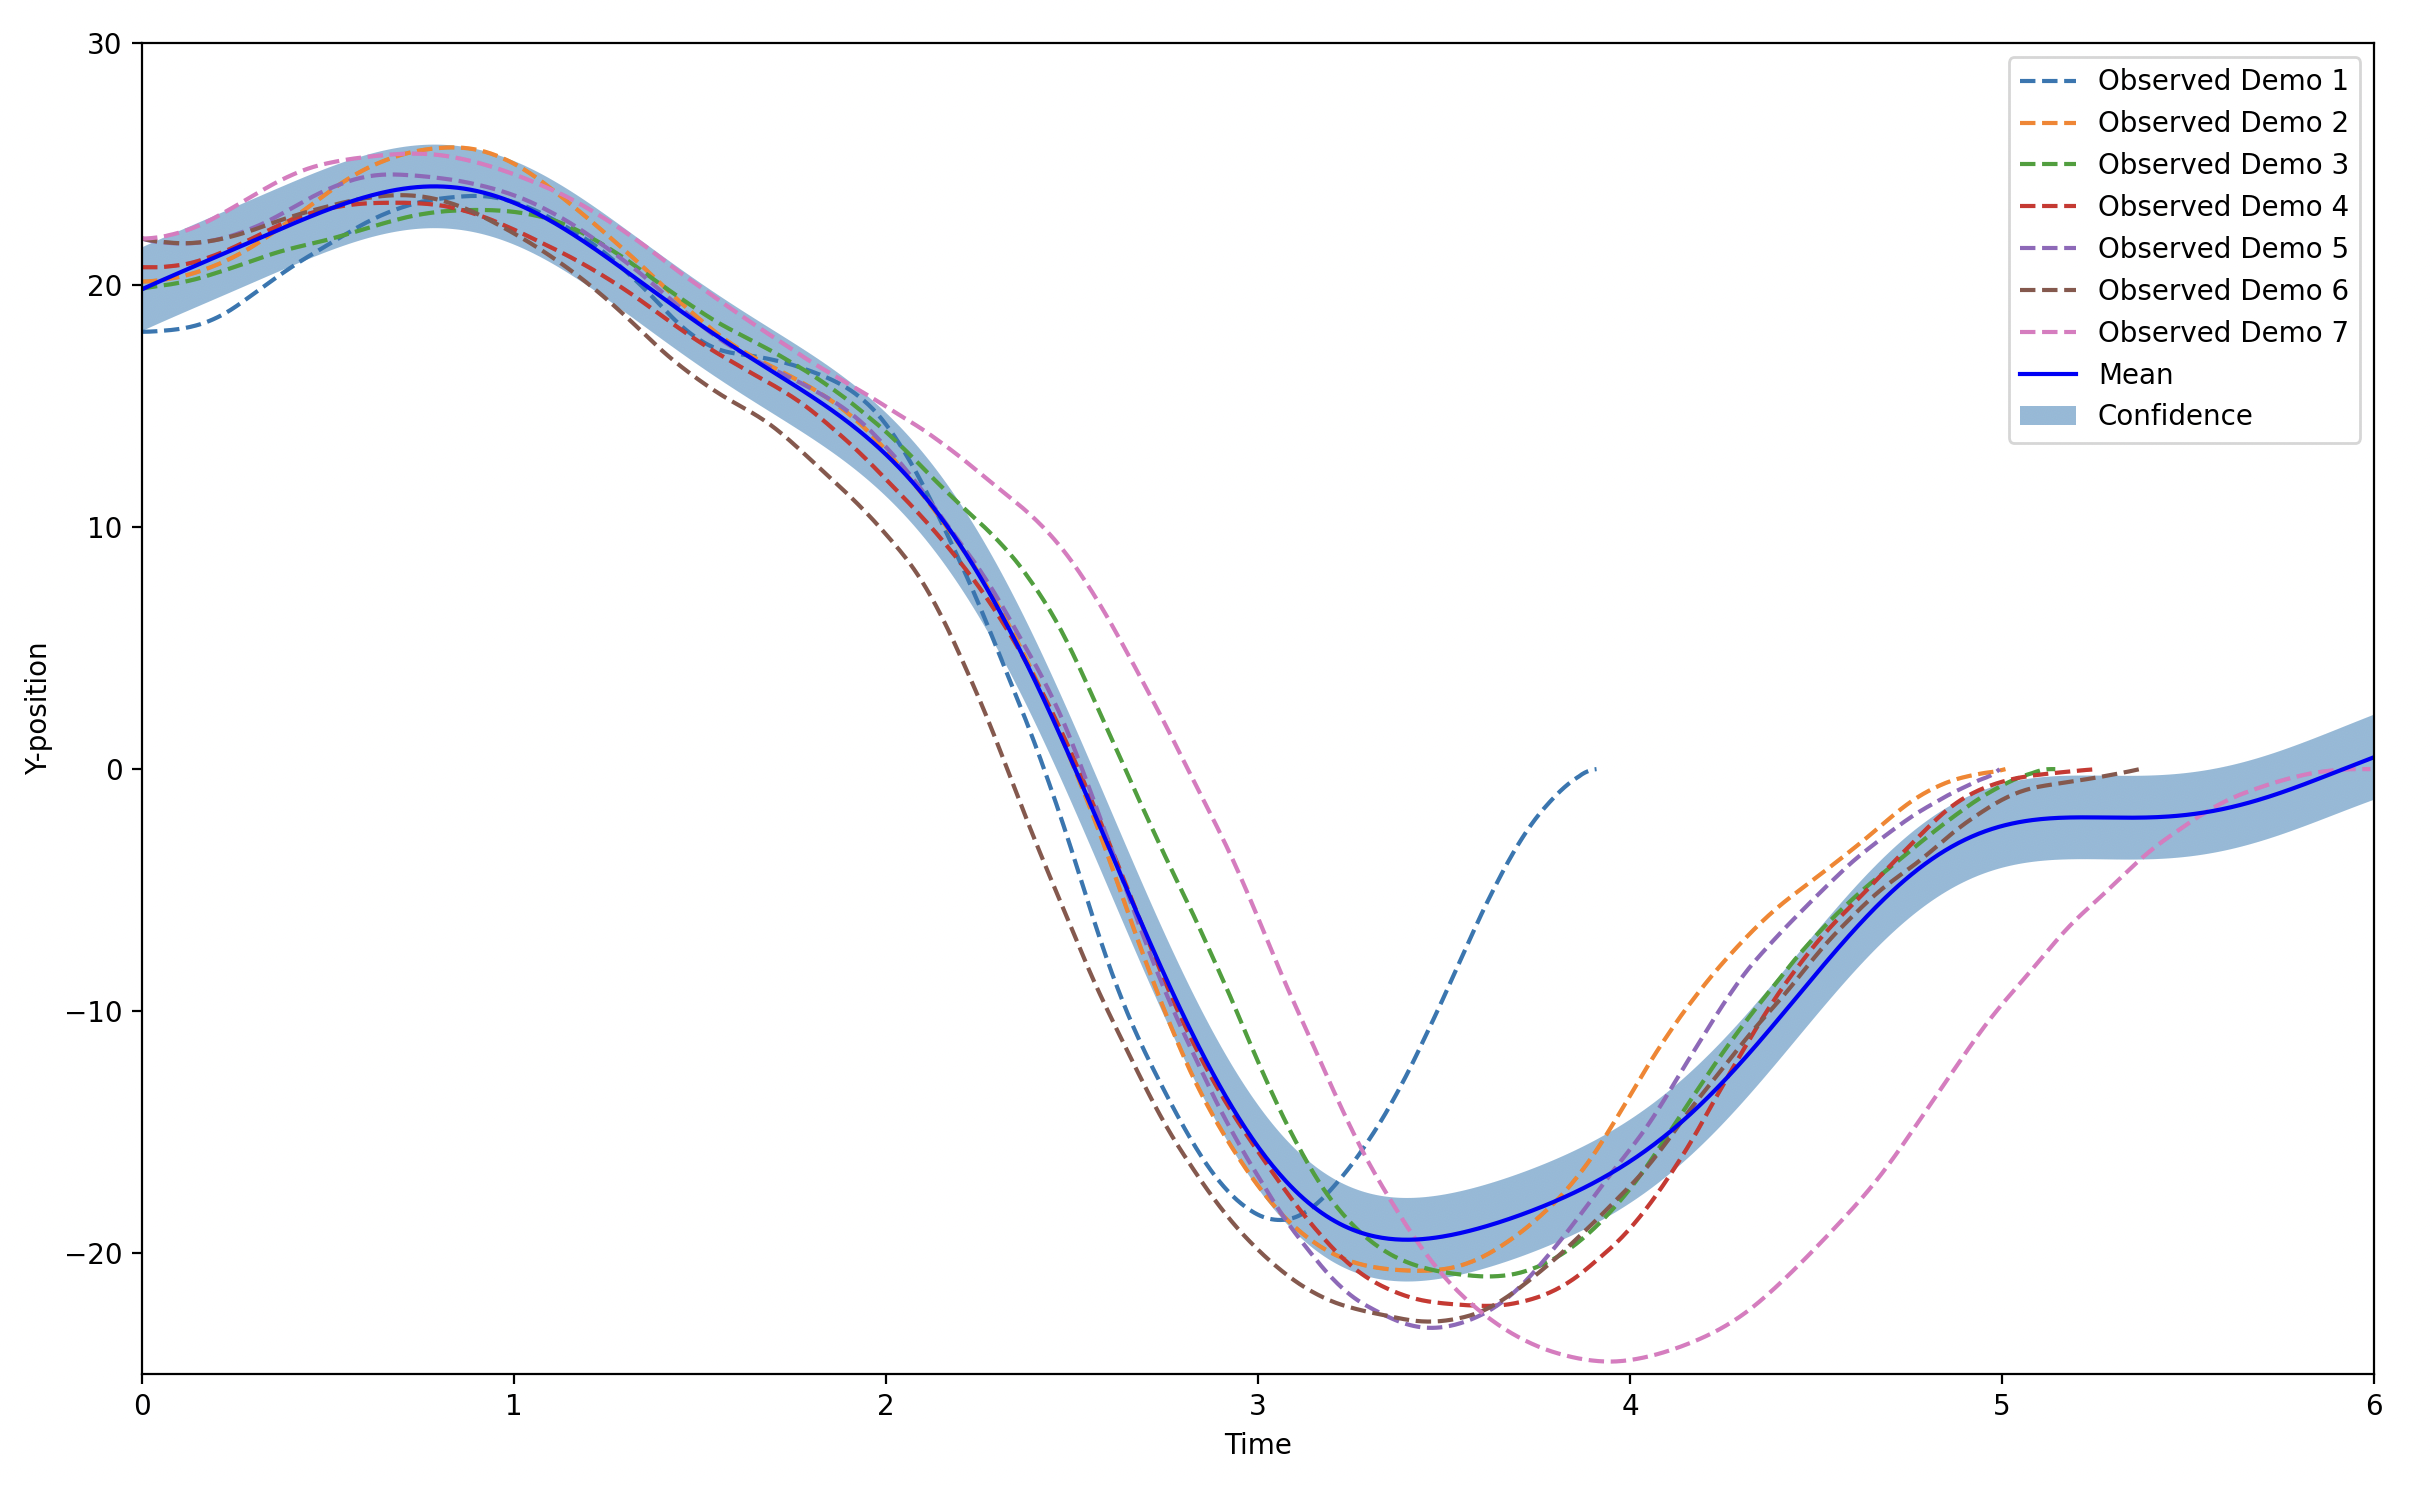
\includegraphics[width=\textwidth]{paper/images/Y_Time_Exact_GP.png}
		\caption{$y$ position as the task (output) and time $t$ as the input to the GP.}
	\end{subfigure}
	
	\caption{The 7 trajectories of the "heee" motion shape are shown in various colors. The posterior mean and confidence region are shown as the blue line and the blue shaded region respectively.}

    \label{fig:scalar_exact}

    \vspace{-2em}
\end{figure*}

\subsection{Trajectory Estimation}
We use the Radial Basis Function (RBF) kernel function in all of the following Gaussian Processes.

\begin{figure*}[t!]
    \captionsetup{font=footnotesize}
    \centering
    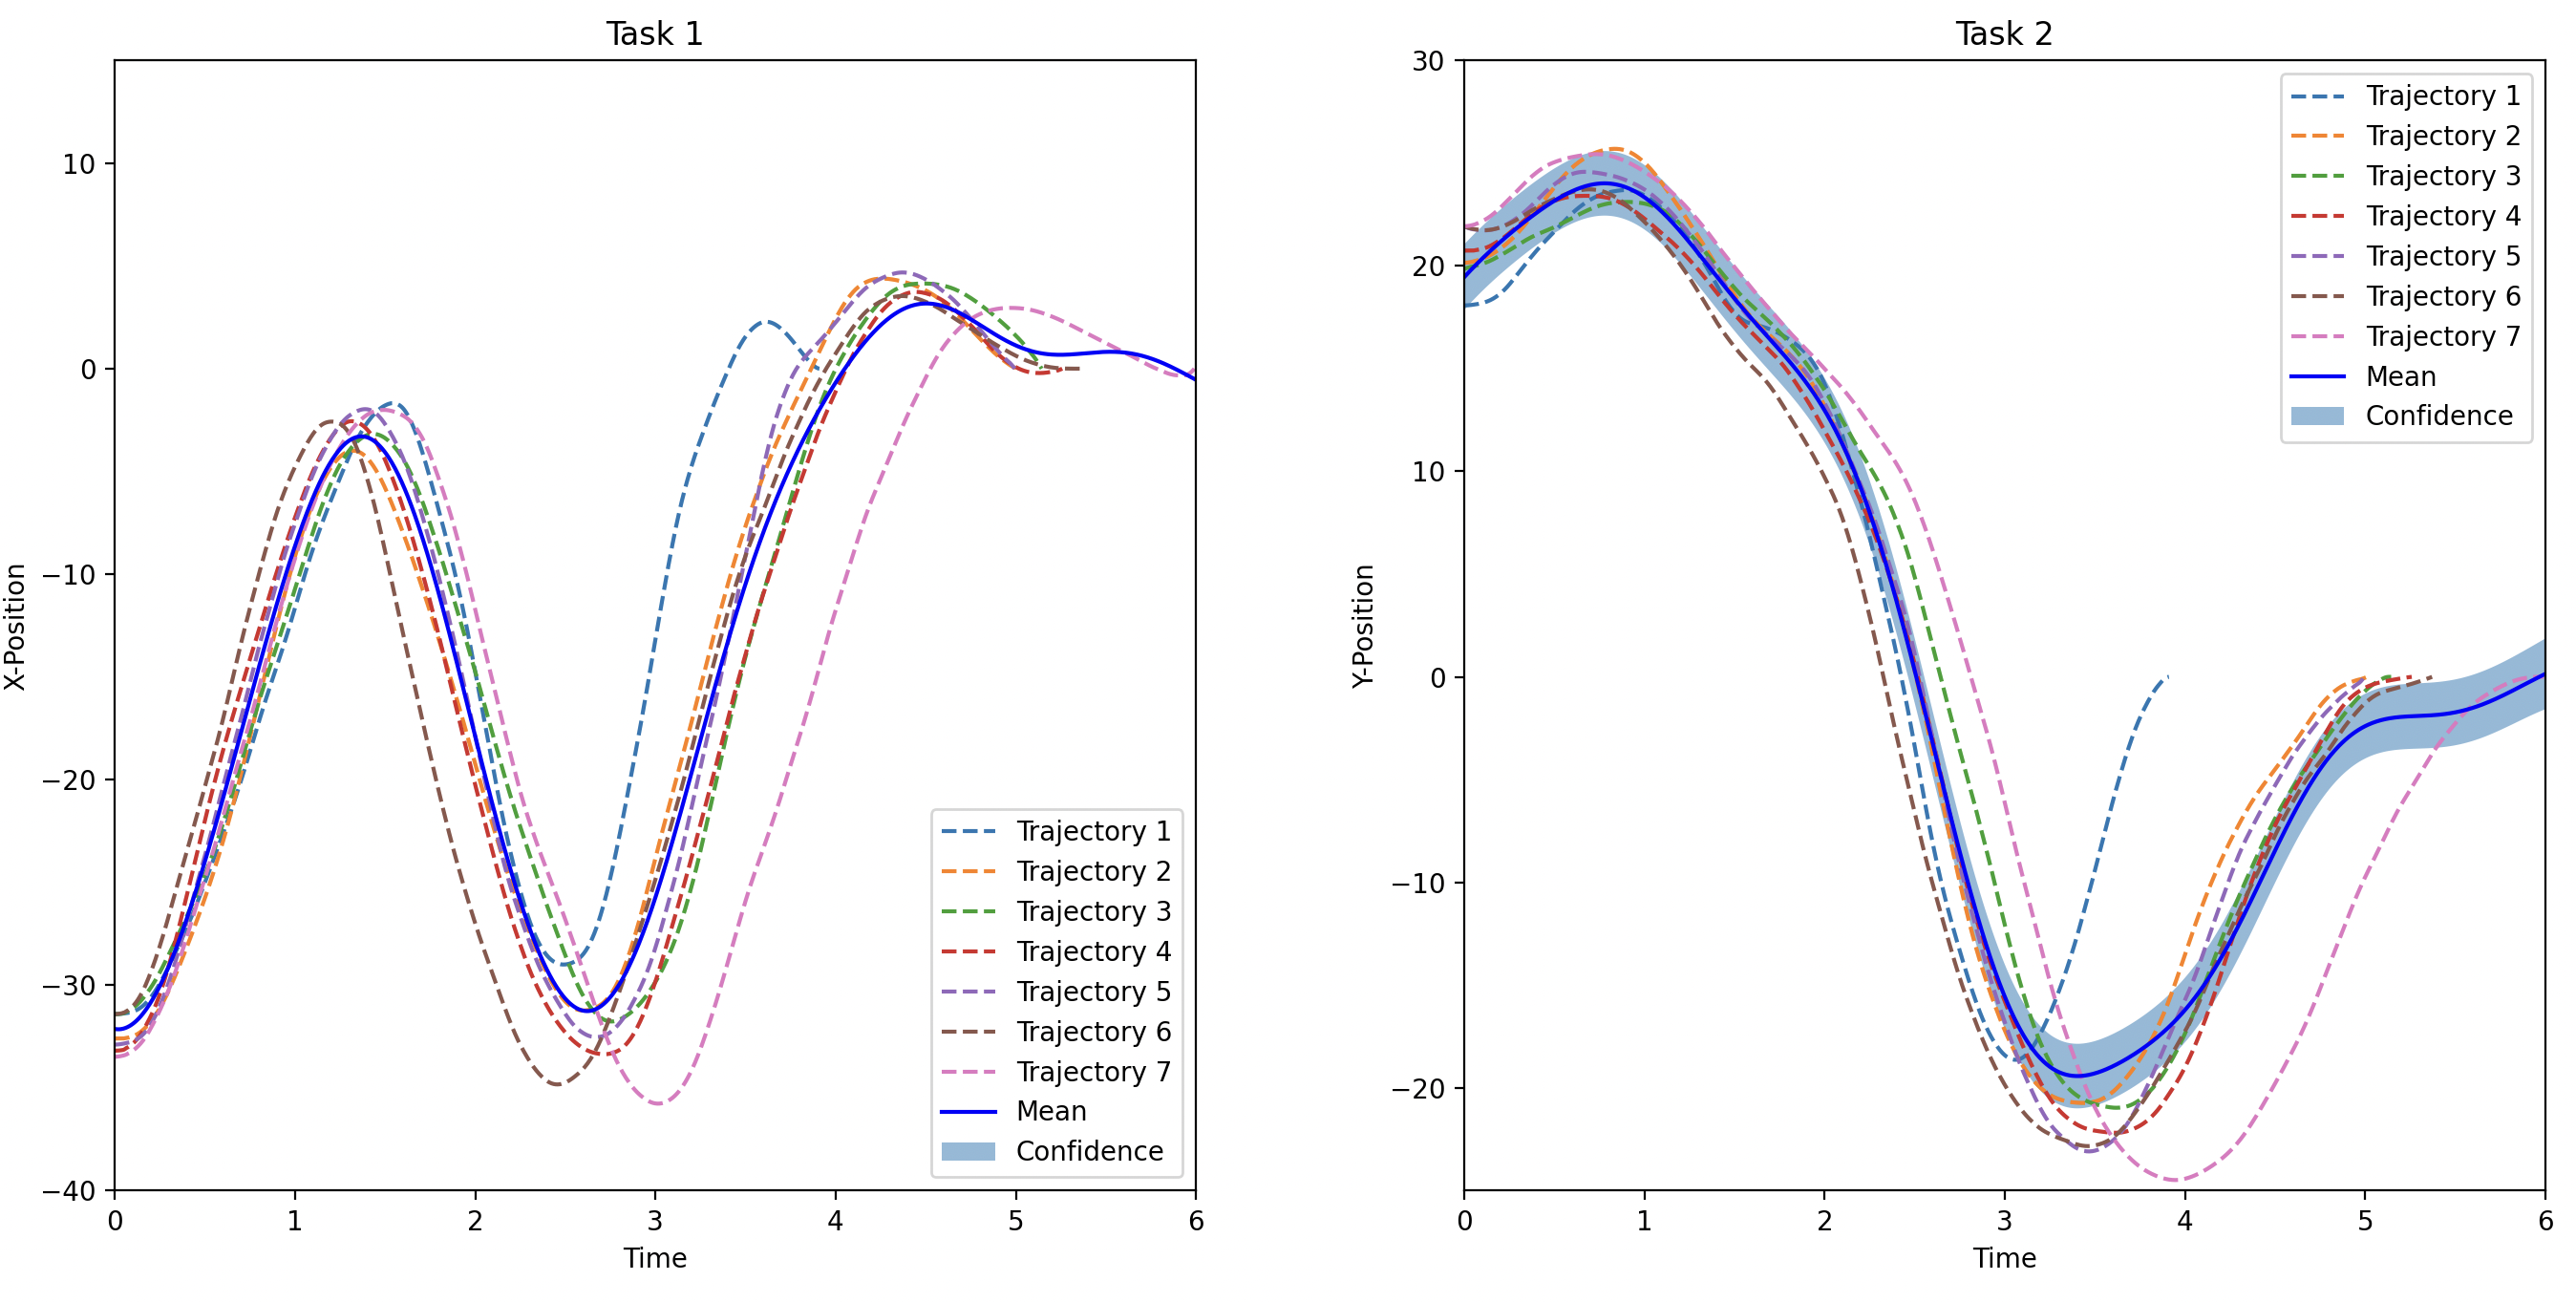
\includegraphics[width=\textwidth]{paper/images/Multi_Exact_GP.png}
    \caption{An example of 10 trajectories sampled from the posterior of the variational multi-output Gaussian process.}
    \label{fig:multitask_exact}
    \vspace{-2em}
\end{figure*}

\subsubsection{Gaussian Process with Exact Inference}
The Gaussian Process with exact inference can only map single-dimensional input to a single-dimensional output. Therefore, two Gaussian Processes were trained independently for predicting $x$-position from time input and $y$-position from time input. Figure~\ref{fig:scalar_exact} 1a shows the 7 trajectories of the "heee" motion shape for $x$ position as the task and time as input, the mean and the confidence region (two standard deviation above and below the mean). While training independent GPs gave good estimation for the mean and the confidence region, the inter-task covariance information was not encoded which motivated us to experiment with other GPs.

\begin{figure*}[t!]
    \captionsetup{font=footnotesize}
    \centering
    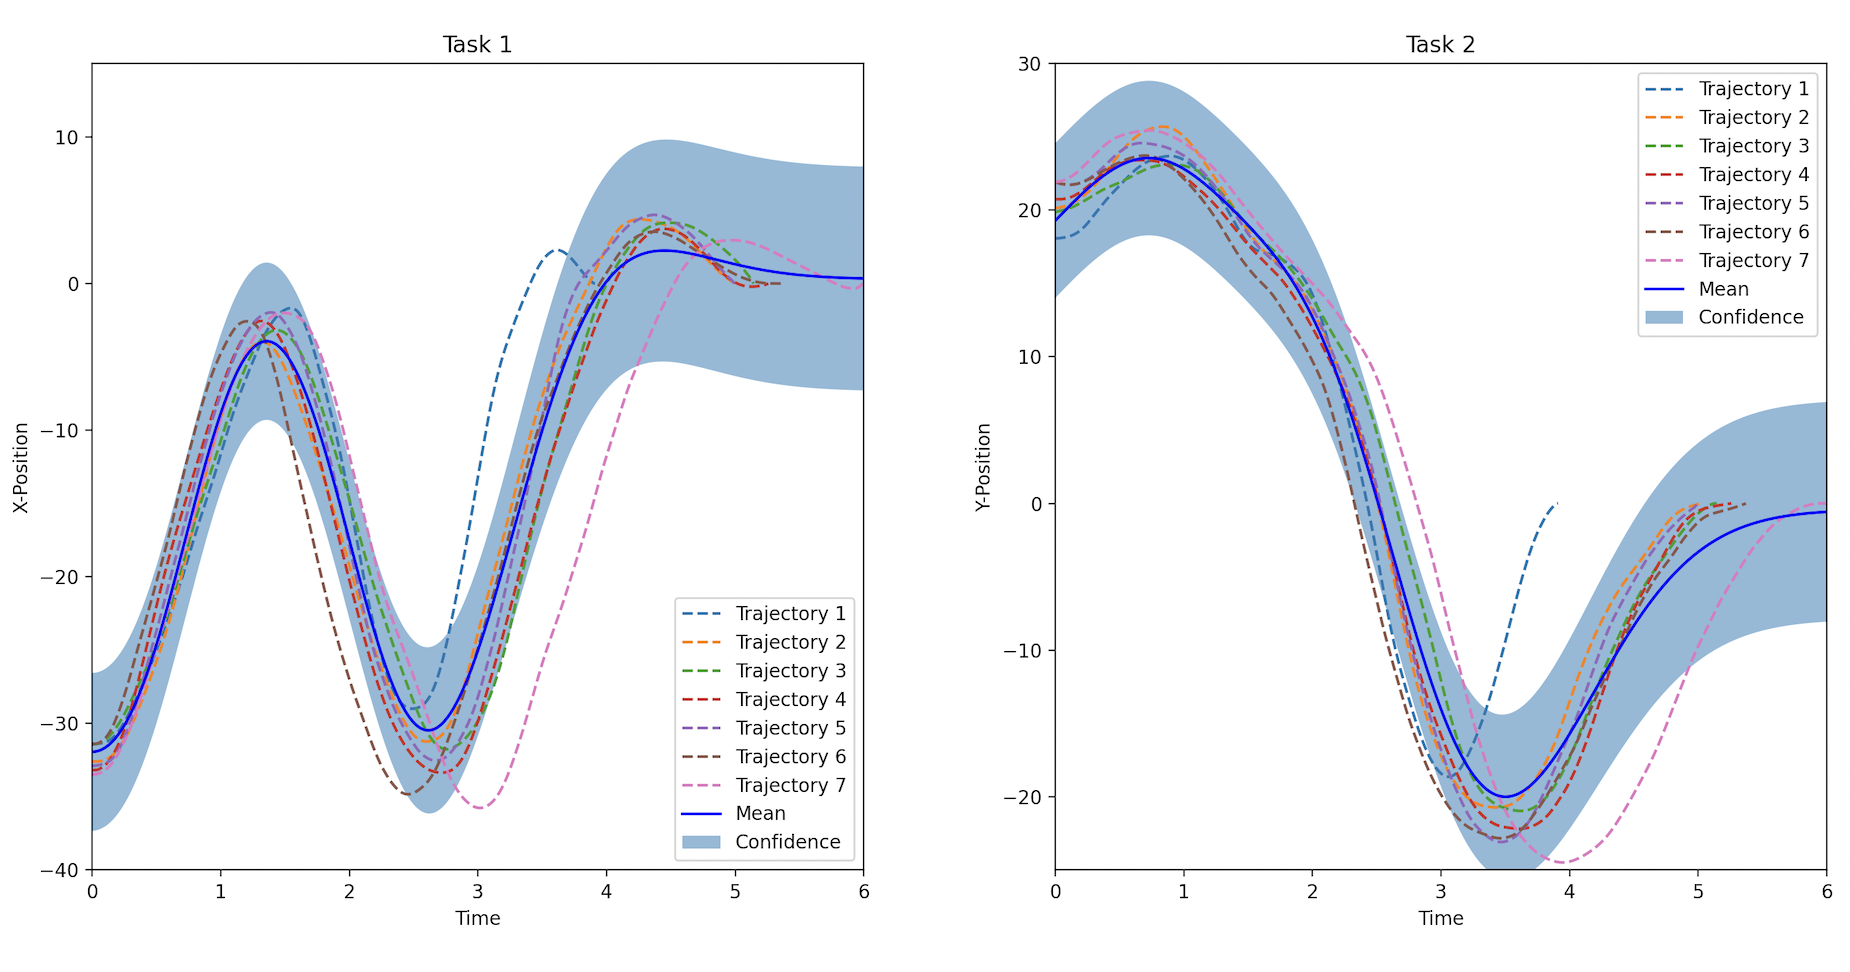
\includegraphics[width=\textwidth]{paper/images/VGP_RBFKernel.png}
    \caption{An example of a multi-output Gaussian process trained to estimate the trajectory distribution via Variational Inference.}
    \label{fig:multitask_approx}
    \vspace{-2em}
\end{figure*}


\begin{figure*}[h!]
    \captionsetup{font=footnotesize}
    \centering
    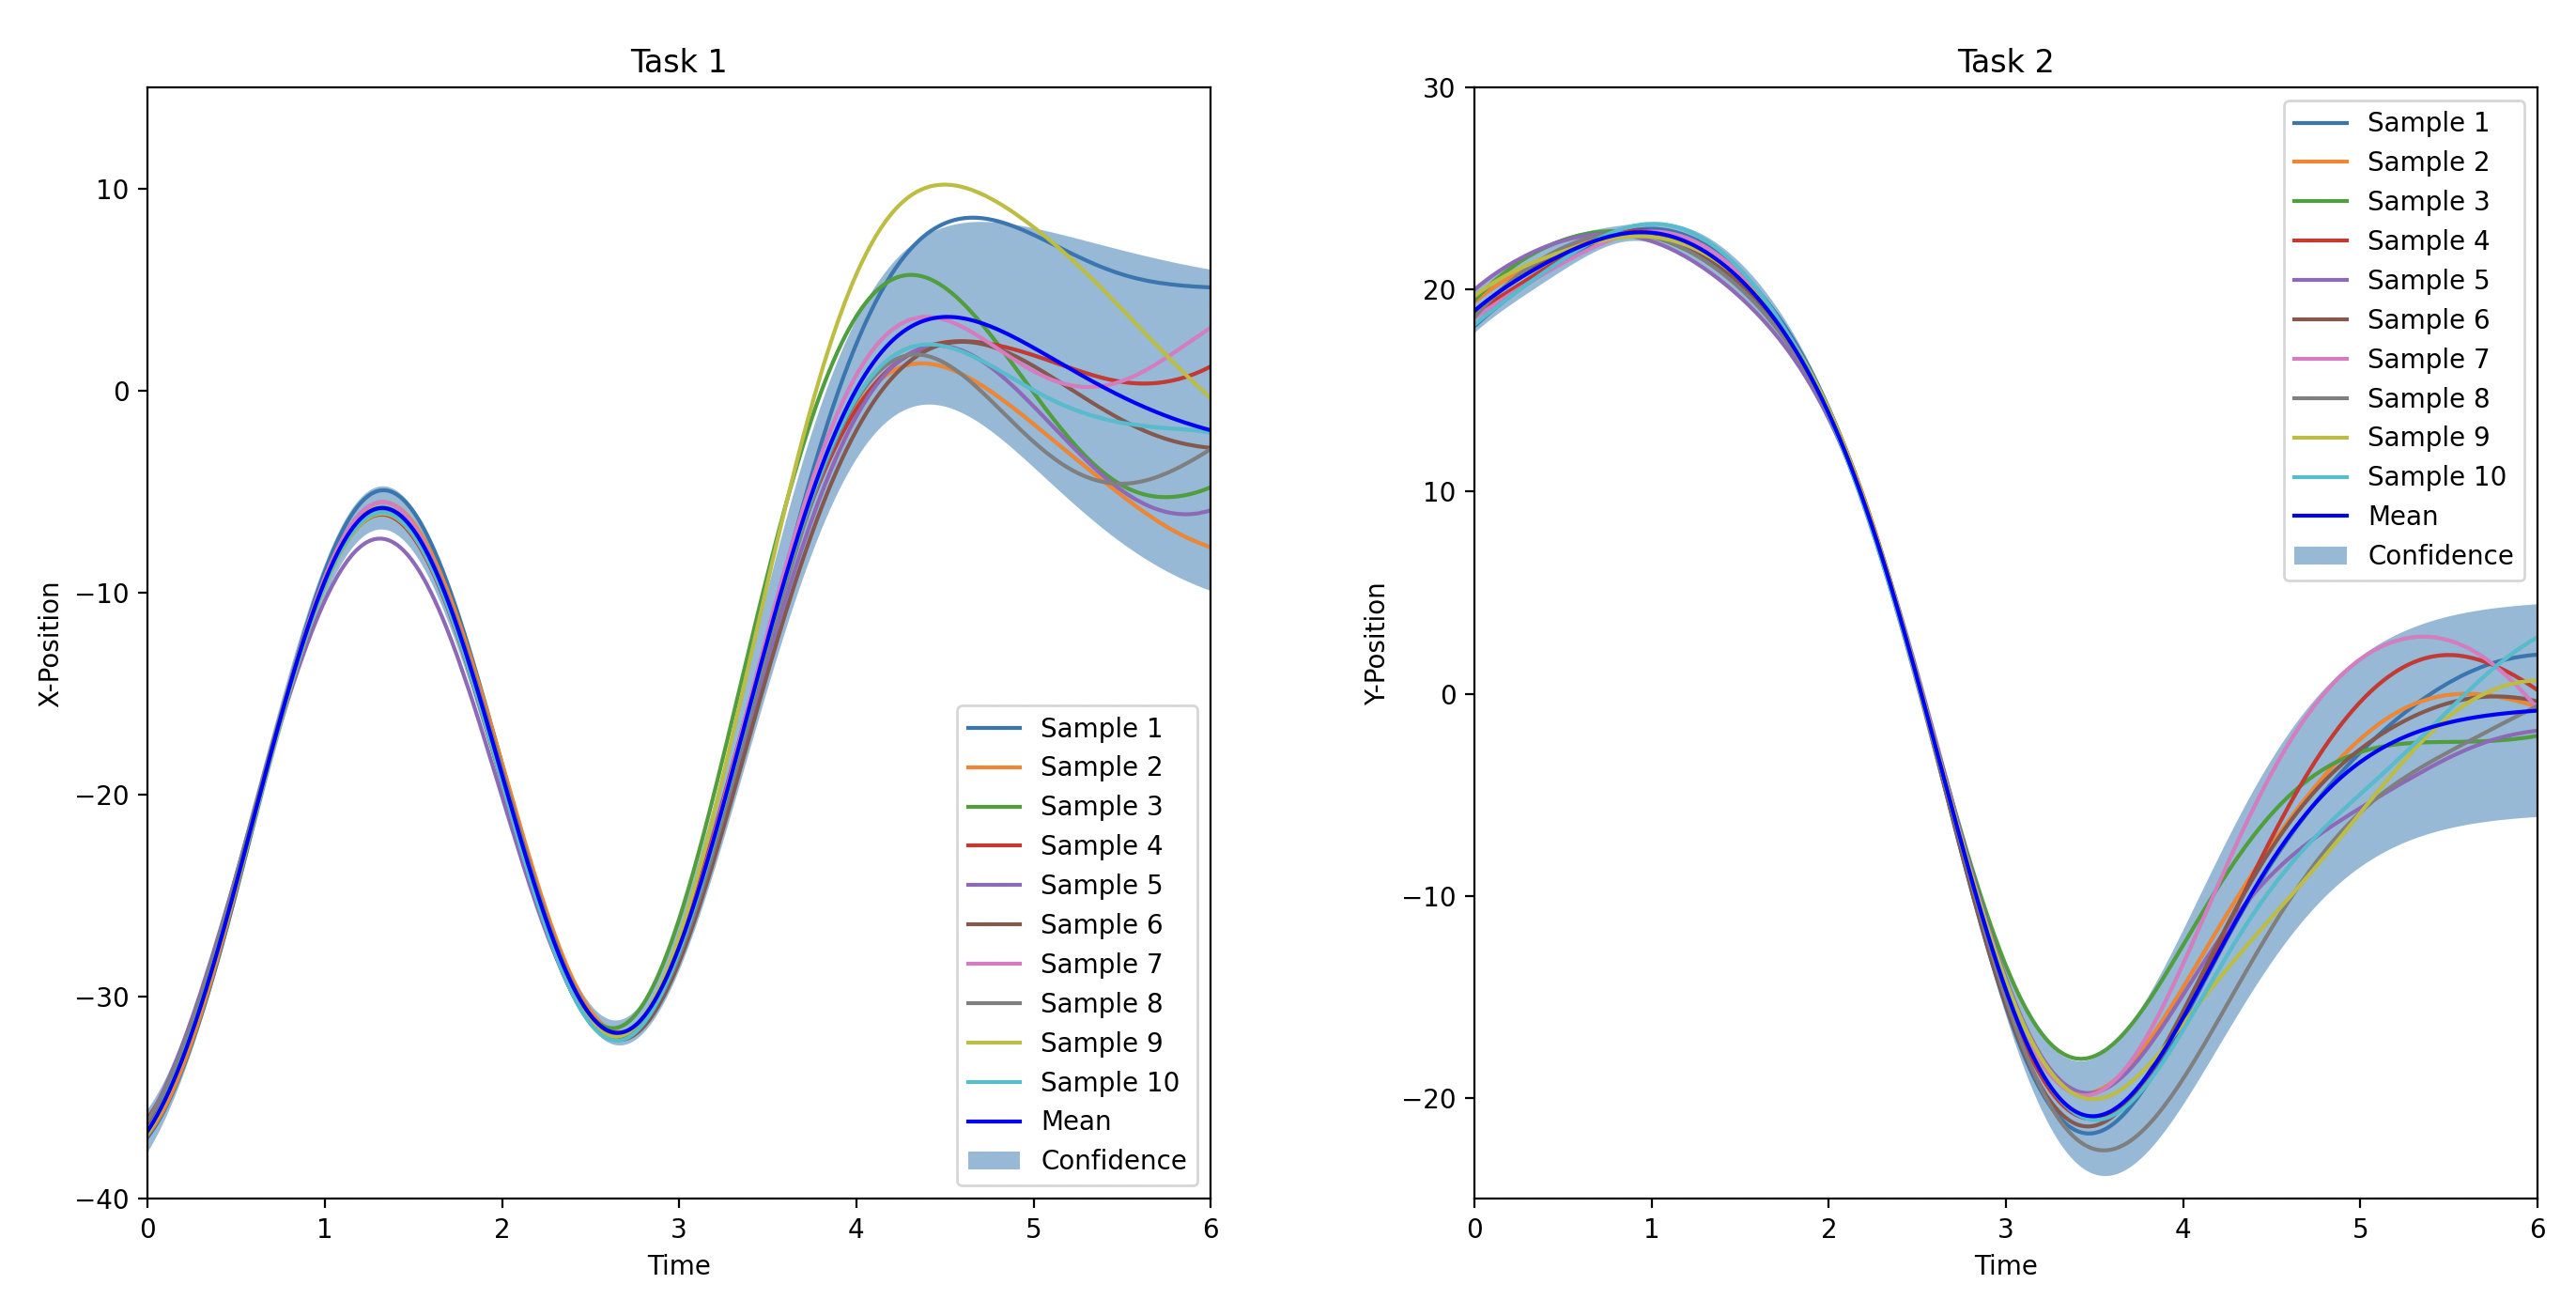
\includegraphics[width=\textwidth]{paper/images/VGP_RBF_sampling.png}
    \caption{An example of 10 trajectories sampled from the posterior of the variational multi-output Gaussian process.}
    \label{fig:multitask_sampling}
    \vspace{-2em}
\end{figure*}

\subsubsection{Multi-Output Gaussian Process with Exact Inference}
The Multi-Output Gaussian Processes can encode the inter-task covariance. We can directly use the time to predict the corresponding X and Y positions. However, due to the large dimensions of the $MN \times MN$ covariance matrix ($14000\times 14000$ in our case), the inverse of the covariance matrix was not being calculated correctly which lead to incorrect confidence values as visible in the left-most plot in Figure~\ref{fig:multitask_exact}. The covariance value was 0 for all pairs of input which lead to no confidence region.


\subsubsection{Variational Multi-Output Gaussian Process}
The Variational Multi-output Gaussian Process uses inducing points to reduce the size of the covariance matrix. We were successfully able to estimate the posterior mean and covariance as shown in Figure~\ref{fig:multitask_approx}. The estimated posterior was sampled to generate near-optimal trajectories (Figure~\ref{fig:multitask_sampling}) which will be used by the RMPFlow to learn the motion policy.

\subsection{Learning RMPs from GP Samples}

\begin{figure}[h!]
    \captionsetup{font=footnotesize}
    \centering
    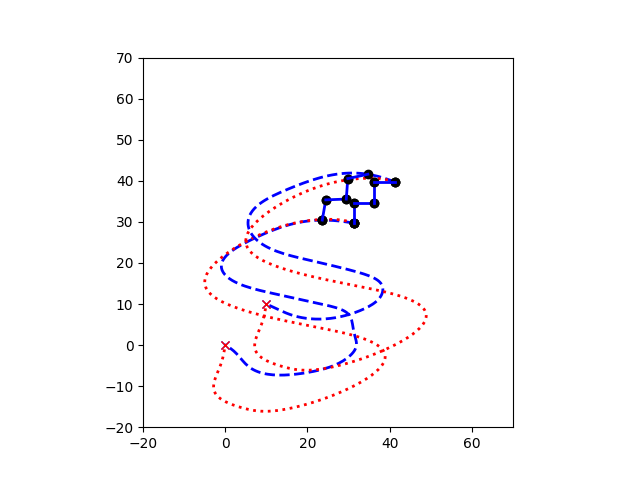
\includegraphics[width=\columnwidth]{paper/images/gp_sample_rmpflow.png}
    \caption{An example of an RMP learned for the ``Sshape'' trajectory in the LASA dataset.}
    \label{fig:gp_rmpflow}
    \vspace{-2em}
\end{figure}

In figure~\ref{fig:gp_rmpflow}, we showcase an example of a learned RMP motion policy which has been trained from samples of the Gaussian Process.
While not quite clean, the general ``S'' structure of the trajectory is reproduced and thus can be counted as a success.
We do believe, however, that there is a bug somewhere in the RMPflow code from the authors of~\cite{Rana20ldc} which we hope to remedy in the near future to generate the expected results.
